\documentclass{article}

\usepackage{a4wide}
\usepackage[utf8]{inputenc}
\usepackage[T1]{fontenc}
\usepackage[french]{babel}
\usepackage[babel=true]{csquotes} % guillemets français
\usepackage{graphicx}
\graphicspath{{Images/}}
\usepackage{color}
\usepackage{hyperref}
\hypersetup{colorlinks,linkcolor=,urlcolor=blue}

\usepackage{amsmath}
\usepackage{amssymb}


\title{Rapport : Gravity Game}
\author{Rococo et Salvan, L3 informatique}
\date{\today}

\begin{document}

\maketitle % pour écrire le titre


%% Le résumé:
\begin{abstract}
  Dans ce rapport écrit en \LaTeX, nous allons vous présenter les caractéristiques de notre application/jeu mobile. Celui-ci existe en 2 versions : une version Android codé en Java et une version iOS codé en Swift. Au début de notre projet, nous avons choisit de faire une application vérifiant le cahier des charges du projet mais pour monter un peu plus en compléxité nous avons décidé de faire un jeu mobile.
 
  Ce jeu se nomme Gravity Ball, il permet au joueur de parcourir  un labyrinthe généré aléatoirement.
\end{abstract}
\newpage
\tableofcontents
\newpage
\section{Introduction}
\label{section:intro} % pour faire référence à la section ailleurs (\ref{...} voir plus bas)
Comme dit juste avant le jeu se nomme Gravity Ball, le joueur parcourt un labyrinthe généré aléatoirement avec l'aide de l'accéléromètre  de téléphone. C'est un jeu qui est très fonctionnel avec le format mobile et parfois ce jeu a était utilisé en tant que mini-jeu dans Zelda Breath of the Wild par exemple ou le gyroscope de la manette permettre à une boule d'atteindre un point objectif.

Après avoir reussi à passer le labyrinthe le joueur peut entrer son pseudo pour ensuite enregistrer son score dans une base de données lui permettant de retrouver son score en seconde. La base de données lui permettra de retrouver ces scores ou celui de ces amis sur son téléphone pour pouvoir se comparer entre eux.

L'application qui est la plus avancé sera la version Android car nous utilisons des environments Windows non propice au développement sur iOS. 

Elle valide les contraintes du cahier des charges demandé :
\begin{itemize}
\item Plusieurs écrans.
\item Plusieurs présentation en forme de liste.
\item Une sauvegarde0/persistance à l'aide d'une base de données.
\item Des contraites pour fonctionner sur tout types d'écran en mode paysage et portrait.
\end{itemize}



\section{Description générale de l'application}
Voici un schèma de notre application: 
\begin{center}
  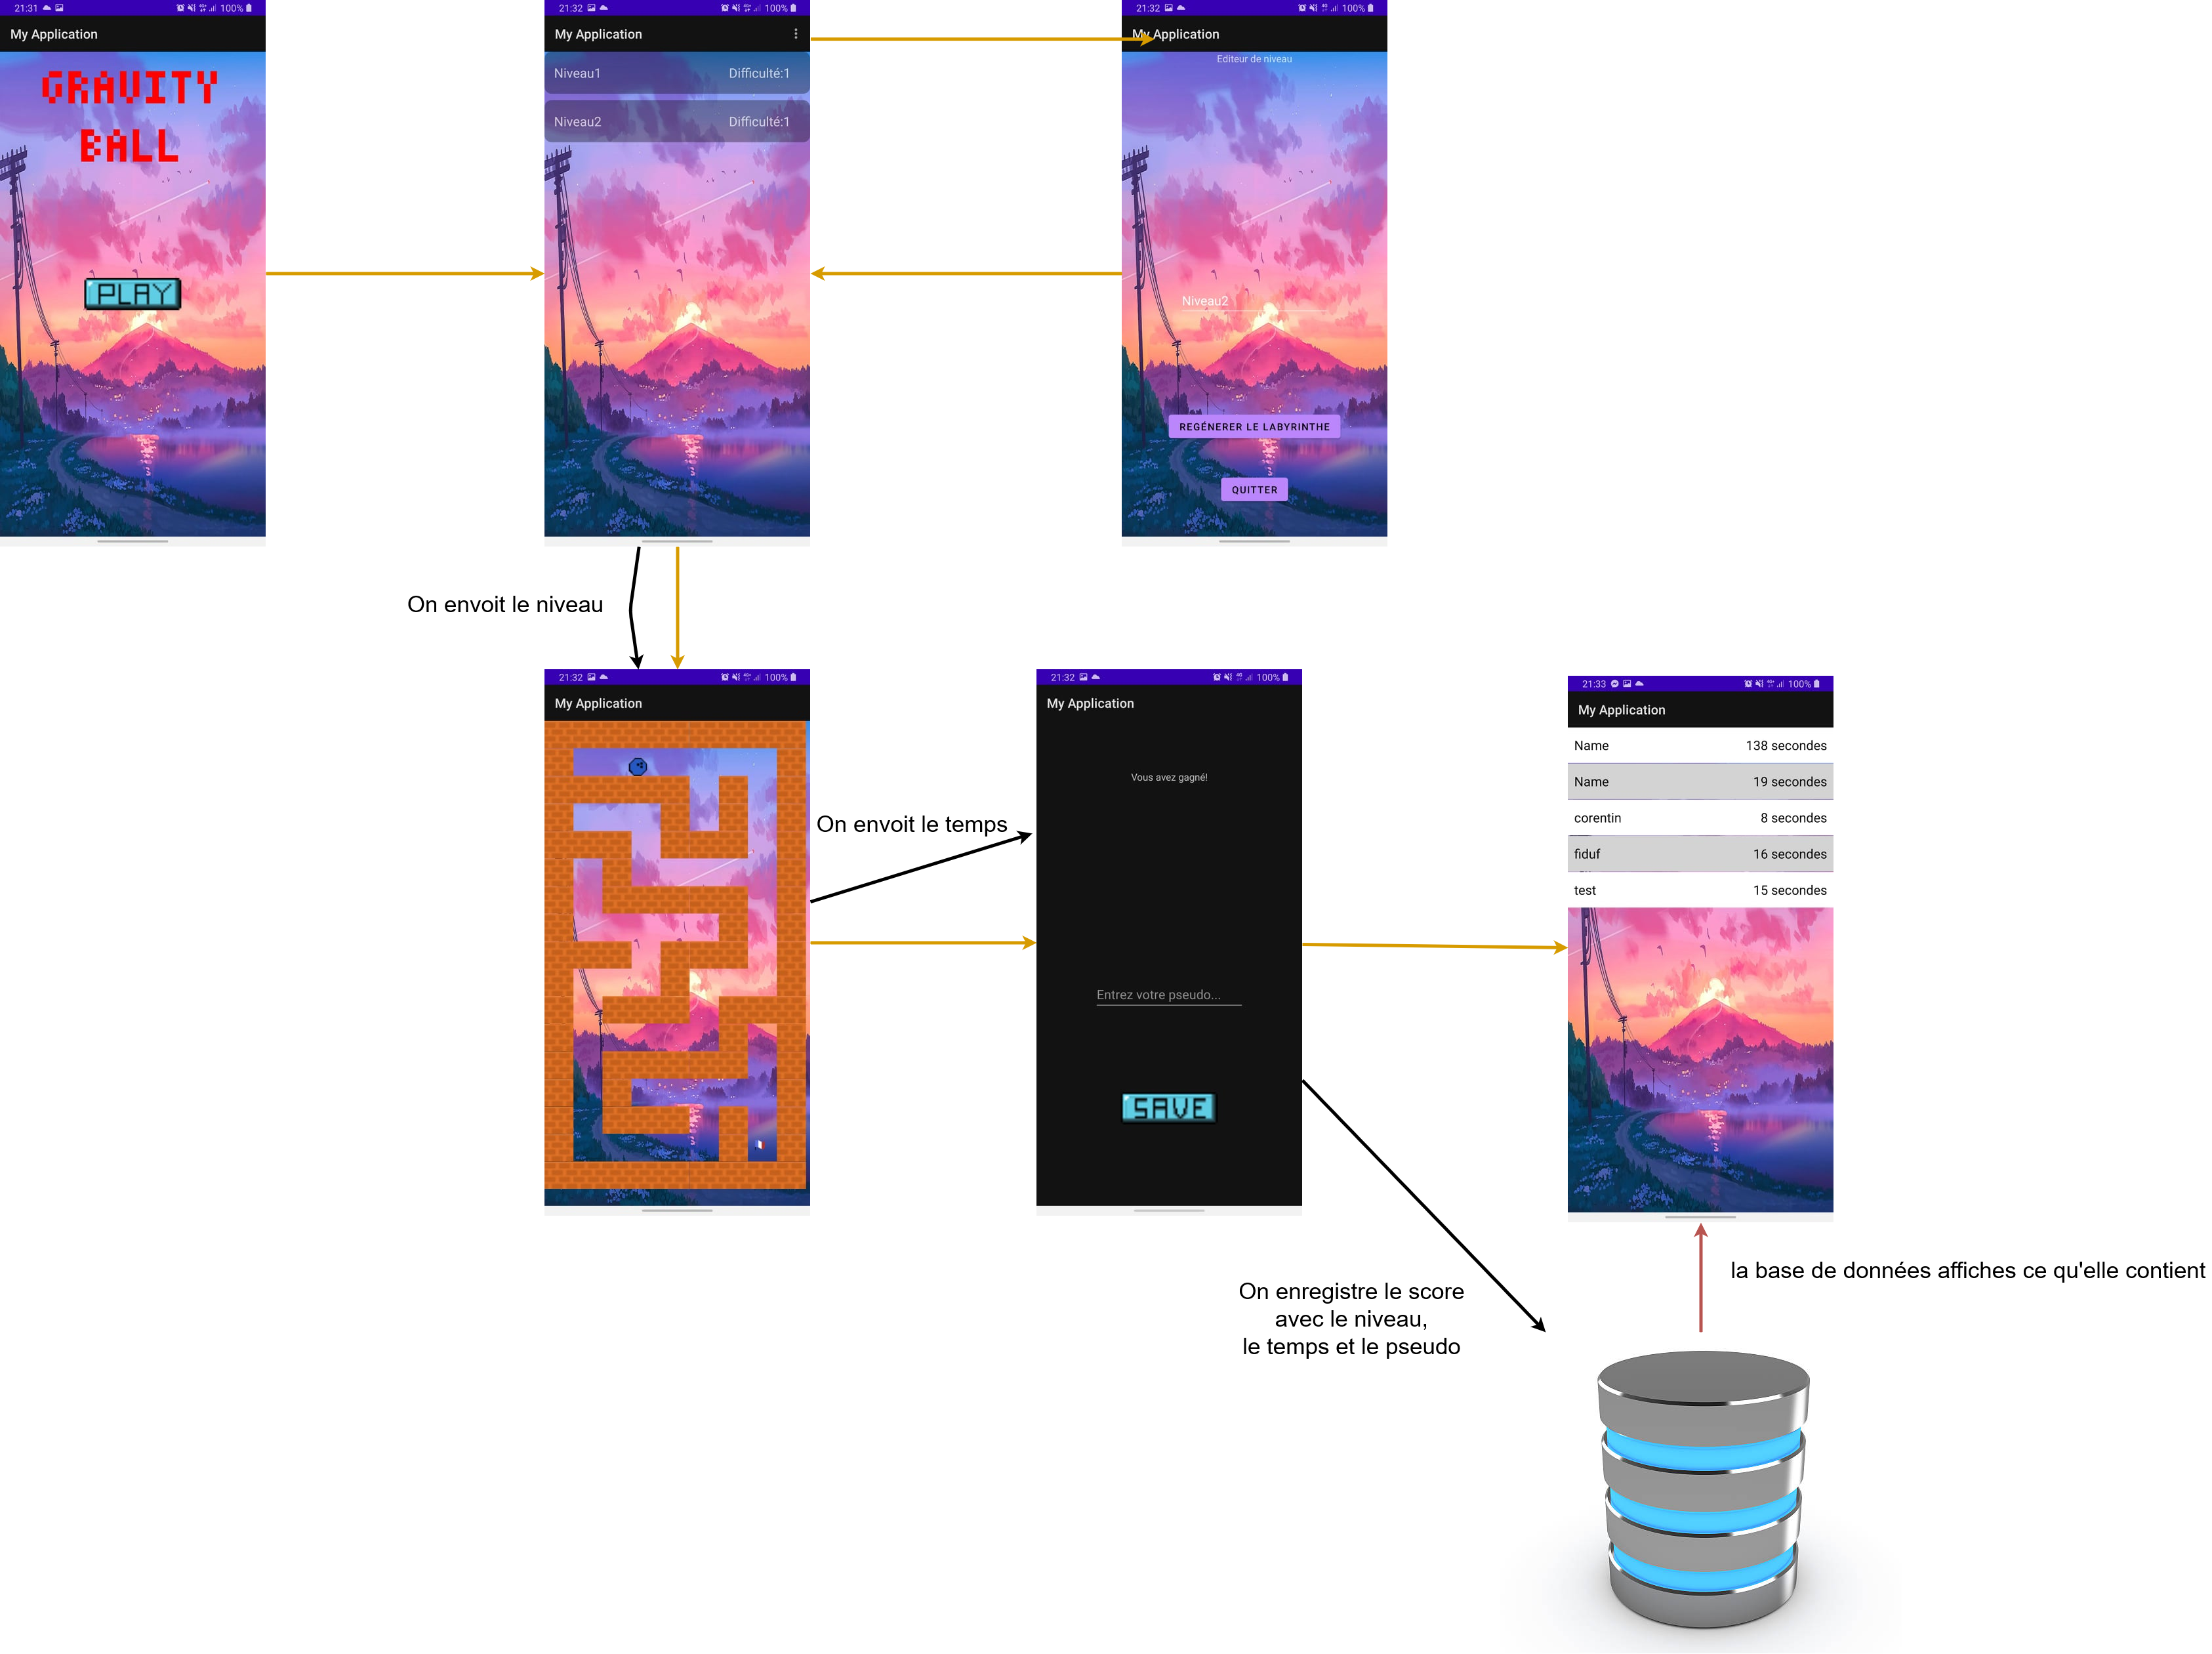
\includegraphics[scale=0.125]{schema.png} % à modifier
\end{center}
\label{section:description}
Le joueur commence en haut à gauche et doit arriver en bas à droit en fonction du labyrinthe. Grâce à l'accéléromètre du téléphone, l'utilisateur peut contrôler la boule pour y arriver. Les collisions avec les murs sont "douces" pour que la balle ne soit pas renvoyer dans tout les sens et lui permettre d'avoir une expérience de jeu confortable, voir même plutôt facile.

Ensuite à la fin du jeu, on enregistre le temps qu'a pris le joueur son pseudo et le niveau dans une base de données pour ensuite l'afficher en fonction du niveau. Les appels de la base de données seront plus tard explicités.

\subsection{Design}
Nous avons gardé un aspect très simple de l'application avec un simple ajout de sprite en pixel art pour l'aspect jeu retro. Cependant il y a un soucis au niveau des sprites car un flou apparait sur chacune d'entres-elles. Les sprites ont été réalisé avec le logiciel Aseprite. L'ajout des sprites a été fait avec l'aide de la documentation Android et de l'utilisation des classes Paint, Canvas et Bitmap. Malheuresement, certains sprites n'ont pas pu être mis en place.
\begin{center}
  
\includegraphics[scale=2]{mur.png}
  
\includegraphics[scale=2]{back.png}
  
\includegraphics[scale=2]{ball.png}
\end{center}
\section{Architecture du code}

\subsection{Android} 
Notre code est plutôt bien construit, surtout au niveau des classes Java. En effet chaque classe possède son fichier et même si une classe comporte une autre classe. Aussi, pour la conception du jeu, nous avons modélisé sa structure avec le langage UML, ensuite nous avons géneré le code java correspondant et l'avons ajouté à notre projet android studio. Nous avons aussi supprimés toute les parties de codes non nécessaires et les fichiers de test ou de 1ère version du projet pour plus de visibilité dans le projet. De plus, nos 16 fichiers java sont nommés de manière à comprendre rapidement la nature des classes manipulés. 
\begin{center}
  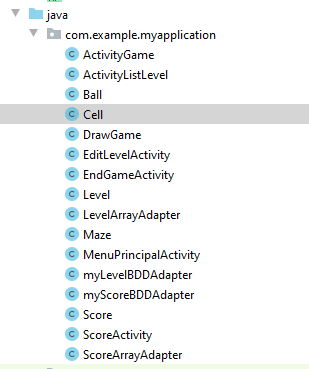
\includegraphics[scale=1]{fichiers.PNG} 
\end{center}
Nos classes peuvent être diviser en 2 "familles" principal :
\begin{itemize}
\item Les classes pour la création du jeu.
\item Les classes pour les différents activités et l'affichage des données.
\end{itemize}
\subsubsection{Création du Jeu}
Pour la création du jeu nous avons : 
\begin{itemize}
\item Ball : la classe qui crée la boule que contrôle le joueur, elle permet de calculer sa nouvelle position de gérer les collisions, sa vitesse mais aussi de vérifier la condition de victoire.
\item Level : la classe qui contient le labyrinthe et qui s'affiche sous forme de liste pour le choix du niveau.
\item Score : classe qui contient le niveau, le temps en secondes et le pseudo du joueur pour être présenter sous forme de liste.
\item Maze : la classe possède comme attribut un tableau à 2 dimensions d'entiers permettant de créer le labyrinthe de manière aléatoire et de gérer l'état de chaque cellule. Pour la génération du labyrinthe, nous utilisons une méthode récursive impliquant un automate cellulaire, nom de l'algorithme:Randomized depth-first search.
\item Cell : Cell est la classe permet de savoir l'état de chaque cellule du tableau d'entiers Maze, la balle pourra savoir si la boule doit entrer en collision, traverser la cellule ou toucher la cellule de victoire. Elle gère aussi l'affichage des cases du labyrinthe
\item DrawGame : permet d'initialiser le jeu c'est à dire la boule, le labyrinthe, l'évolution de la position de la boule et sa condition de victoire.
\end{itemize}
\subsubsection{Gestion des acitivités}
Pour la gestion des activités et l'affichages des données nous avons :
\begin{itemize}
\item MenuPrincipalActivity : qui est l'activité du début.
\item ActivityListLevel : une présentation sous forme de liste qui permet de selectionner ou supprimer un niveau.
\item EditLevelActivity : une activité qui permet de modifier le nom d'un niveau ou de le regénérer. 
\item ActivityGame : une activité qui permet de lancer et initialiser le jeu.
\item EndGameActivity : une activité qui permet de rentrer son pseudo pour enregistrer le score.
\item ScoreActivity : un activité qui permet l'affichage des données.
\end{itemize}
\subsubsection{Persistance et présentation sous formes de listes}
De plus, d'autres fichiers s'y ajoute, ils permettent la persistance des données mais aussi l'affichage des données sous forme de listes.
\begin{itemize}
    \item myScoreBDDAdapter : classe gérant la persistance des données des scores avec l'ajoute dans la base de données et le renvoit de données en fonction d'un paramètre.
    \item myScoreBDDAdapter : classe gérant la persistance des données des levels avec l'ajoute dans la base de données et le renvoit de données en fonction de paramètre(abandonner à cause de la compléxité de stoker la classe Maze).
    \item ScoreArrayAdapter : classe permettant l'affichage des données dans un LinearLayout.
    \item LevelArrayAdapter : classe permettant l'affichage des données dans un LinearLayout.
\end{itemize}
\subsubsection{Points importants de l'application}
Voyons maintenant des points importants de notre programme Android :
\begin{itemize}
\item L'utilisation de l'accéléromètre et fin du jeu en cas si la condition de victoire est validé:
Un smartphone possède plusieurs capteurs permettant d'augmenter les intercations, parmi ces capteurs, nous retrouvons l'accéléromètre qui récupère l'acceleration subit par le smartphone dans les 3 dimensions de l'espace:
    \begin{figure}[h!]
        \begin{center}
        \begin{tabular}{|l|l|}
        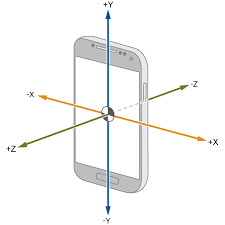
\includegraphics[scale=0.6]{schemaAccelerometre.png} %l'image est réduite de moitié
        \end{tabular}
        \end{center}
        \caption{Axes pris en compte par l'accéléromètre}
        \label{tab:Schema electrique}
    \end{figure}
    Grâce à ce capteur nous récupérons une composante importante dans la réalisation de notre jeu, la gravité. En effet elle est appliqué dans la même direction peut importe l'orientation du smartphone. Afin de simuler au l'impression de contrôler une vrai boule sur un plateau, nous appliquons la même force de gravité que la Terre sur la boule. Comme le jeu se joue en 2 dimensions, seul deux axes sont à prendre en compte. D'après la figure 1, les axes Z et X seront retenus.
    
    Pour mouvoir la boule, nous devons interpréter cette accélération. Grâce à la mécanique newtonienne qui nous dit que l'integrale de l'accéleration par rapport au temps est égal à la vitesse et que l'integral de la vitesse par rapport au temps est égal à la position, nous appliquons successivement ces opération afin d'obtenir des coordonnées qui serviront à mettre à jour la position de la balle au cours du temps.
    \begin{verbatim}
        public class ActivityGame extends AppCompatActivity implements SensorEventListener {
    public static final String EXTRA_TEMPS = "EXTRA_TEMPS";
    public static final String EXTRA_NIVEAU2 = "EXTRA_NIVEAU";
    private Handler mHandler = new Handler();
    public static int i = 0;
    private View a;
    public SensorManager sensorManager;
    public Sensor sensor;
    public static float[] gravity = new float[3];
    public static float[] linear_acceleration = new float[3];
    long debut = System.currentTimeMillis();
    @Override
    protected void onCreate(Bundle savedInstanceState) {
        super.onCreate(savedInstanceState);
        setContentView(R.layout.activity_draw_game);

        a= (View) findViewById(R.id.viewGame);
        sensorManager = (SensorManager) getSystemService(SENSOR_SERVICE);
        sensorManager.registerListener(this,sensorManager.getDefaultSensor(Sensor.TYPE_ORIENTATION),
                Sensor.TYPE_ACCELEROMETER);

        DrawGame.currentLevel= ActivityListLevel.listLevel.get(ActivityListLevel.currentLevel);

    }
    public void onSensorChanged(SensorEvent event){
        // In this example, alpha is calculated as t / (t + dT),
        // where t is the low-pass filter's time-constant and
        // dT is the event delivery rate.
        double alpha = 0.1;
        i = i+1;
        // Isolate the force of gravity with the low-pass filter.
        gravity[0] = (float)(alpha) * gravity[0] + (1 - (float)(alpha)) * event.values[0];
        gravity[1] = (float)(alpha) * gravity[1] + (1 - (float)(alpha)) * event.values[1];
        gravity[2] = (float)(alpha) * gravity[2] + (1 - (float)(alpha)) * event.values[2];

        // Remove the gravity contribution with the high-pass filter.
        linear_acceleration[0] = event.values[0] - gravity[0];
        linear_acceleration[1] = event.values[1] - gravity[1];
        linear_acceleration[2] = event.values[2] - gravity[2];
        if(DrawGame.currentLevel.mazeLevel != null) {
            if (DrawGame.ball.isWinned(DrawGame.currentLevel.mazeLevel)) {
                Intent intentbefore = getIntent();
                String niveau = intentbefore.getStringExtra(ActivityListLevel.EXTRA_NIVEAU);
                long tempsEcoulMills = (System.currentTimeMillis() - debut)/1000;
                String temps = String.valueOf(tempsEcoulMills) +" secondes";
                Intent intent = new Intent(this, EndGameActivity.class);
                intent.putExtra(EXTRA_TEMPS,temps);
                intent.putExtra(EXTRA_NIVEAU2,niveau);
                startActivity(intent);
                System.exit(0);

            }
        }
        a.invalidate();
    }
    \end{verbatim}
    
    \item La classe DrawGame qui permet d'initialiser les objets utilisés dans le jeu :
\begin{verbatim}
public class DrawGame extends View {

    static Ball ball= new Ball(0,0, 30);
    static Level currentLevel;
    public DrawGame(Context context,  AttributeSet attrs) {
        super(context, attrs);

    }
    @Override
    protected void onDraw(Canvas canvas) {
        currentLevel.mazeLevel.initGrid(getWidth(), getHeight());
        ball.size= getHeight()/currentLevel.h/3;
        Paint paint = new Paint();
        currentLevel.mazeLevel.affiche(canvas, paint);
        Ball.affiche(paint, canvas,this.getContext());
        paint.setStyle(Paint.Style.FILL);
        Ball.updatePosition( (ActivityGame.gravity[1]),  (ActivityGame.gravity[2]), getWidth(), getHeight(), currentLevel.w, currentLevel.h);
        Ball.collision(paint, canvas, currentLevel.mazeLevel);
        Ball.isWinned(currentLevel.mazeLevel);
        super.onDraw(canvas);
    }

}

\end{verbatim}
\item La récuperation de données d'une autre activité et le passage vers une autre activité avec envoi de données, nous nous sommes aidés du site OpenClassroom expliquant à merveille comment utiliser la classe Intent :
\begin{verbatim}
    public class EndGameActivity extends AppCompatActivity {
    public static final String EXTRA_PSEUDO = "EXTRA_PSEUDO";
    public static final String EXTRA_TEMPS2 = "EXTRA_TEMPS2";
    public static final String EXTRA_NIVEAU3 = "EXTRA_NIVEAU3";
    EditText editText;
    String pseudo;
    @Override
    protected void onCreate(Bundle savedInstanceState) {
        super.onCreate(savedInstanceState);
        setContentView(R.layout.activity_end_game);
        editText = (EditText) findViewById(R.id.editTextTextPersonName2);

    }


    public void GoScore (View view){
        pseudo = editText.getText().toString();
        Intent intentbefore = getIntent();
        String temps = intentbefore.getStringExtra(ActivityGame.EXTRA_TEMPS);
        String niveau = intentbefore.getStringExtra(ActivityGame.EXTRA_NIVEAU2);
        Intent intent = new Intent(this,ScoreActivity.class);
        intent.putExtra(EXTRA_TEMPS2,temps);
        intent.putExtra(EXTRA_PSEUDO, pseudo);
        intent.putExtra(EXTRA_NIVEAU3,niveau);
        startActivity(intent);
    }
}
\end{verbatim}
\ La récupération de données pour ensuite les stocker dans la base de données et les affichers en fonction d'un paramètre :
\begin{verbatim}
    public class ScoreActivity extends AppCompatActivity {
    public static  int id = 0;
    private ListView mListView;
    private ScoreArrayAdapter mAdapter;
    private myScoreBDDAdapter bdAdapter;
    public static ArrayList<Score> listscores = new ArrayList<Score>();

    @Override
    protected void onCreate(Bundle savedInstanceState) {
        //ScoreBDD Scorebdd = new ScoreBDD(this);
        //Scorebdd.open();
        bdAdapter = new myScoreBDDAdapter(this);
        bdAdapter.open();
        // on reprends l'intention
        Intent intentbefore = getIntent();
        String pseudo = intentbefore.getStringExtra(EndGameActivity.EXTRA_PSEUDO);
        System.out.println(pseudo);
        String temps = intentbefore.getStringExtra(EndGameActivity.EXTRA_TEMPS2);
        System.out.println(temps);
        String niveau = intentbefore.getStringExtra(EndGameActivity.EXTRA_NIVEAU3);
        System.out.println(niveau);
        super.onCreate(savedInstanceState);
        bdAdapter.insertScore(pseudo,temps,niveau);
        //bdAdapter.insertScore("CORENTIN","CORENTIN","CORENTIN");
        //listscores.add(new Score(23,"jojo","300","3"));
        //listscores.add(new Score(2,"jajaja","301","3"));
        setContentView(R.layout.activity_main);
        mListView = (ListView) findViewById(R.id.list);

        mAdapter = new ScoreArrayAdapter(this, bdAdapter.getScorebyLevel(niveau));
        mListView.setAdapter(mAdapter);

    }
\end{verbatim}
\end{itemize}
\subsection{iOS}
Pour développer l'application sur iOS, nous avons traduit nos classes Java en classe Swift manuellement, donc on y retrouve certains classes pour la création du jeu.Malgré le fait que le projet iOS ne soit pas fini, il comporte les points du cahier des charges :
\begin{itemize}
    \item Plusieurs écrans.
    \item Une présentation sous formes de listes.
    \item Des contraites pour fonctionner en format paysages et portrait.
\end{itemize}
L'application iOS comporte des segues permettant le transfert de données entre controlleurs :
\begin{verbatim}
    override func prepare(for segue: UIStoryboardSegue, sender: Any?) {
        if segue.identifier == "showDetail" {
            if let indexPath = tableView.indexPathForSelectedRow {
                let object = objects[indexPath.row]
                let controller = (segue.destination as! UINavigationController).topViewController as! DetailViewController
                controller.detailItem = object
                controller.navigationItem.leftBarButtonItem = splitViewController?.displayModeButtonItem
                controller.navigationItem.leftItemsSupplementBackButton = true
                detailViewController = controller
            }
        }
    }
\end{verbatim}
Notre application inclus aussi une présentation sous formes de listes :
\begin{verbatim}
    
    override func numberOfSections(in tableView: UITableView) -> Int {
        return 1
    }

    override func tableView(_ tableView: UITableView, numberOfRowsInSection section: Int) -> Int {
        return objects.count
    }

    override func tableView(_ tableView: UITableView, cellForRowAt indexPath: IndexPath) -> UITableViewCell {
        let cell = tableView.dequeueReusableCell(withIdentifier: "Cell", for: indexPath)
        let object = objects[indexPath.row]
        cell.textLabel!.text = object.levelName
        return cell
    }

    override func tableView(_ tableView: UITableView, canEditRowAt indexPath: IndexPath) -> Bool {
        // Return false if you do not want the specified item to be editable.
        return true
    }

    override func tableView(_ tableView: UITableView, commit editingStyle: UITableViewCell.EditingStyle, forRowAt indexPath: IndexPath) {
        if editingStyle == .delete {
            objects.remove(at: indexPath.row)
            tableView.deleteRows(at: [indexPath], with: fade)
        } else if editingStyle == .insert {
            // Create a new instance of the appropriate class, insert it into the array, and add a new row to the table view.
        }
    }
}
\end{verbatim}
Et comme en Java, notre programme permet de créer des labyrinthes aléatoire avec la classe Maze comme le montre cette fonction de Maze :
\begin{verbatim}
     func regenerate()
    {
        self.h = Float(h);
        self.w = Float(w);
        for i in 0...Int(h)
        {
            for j in 0...Int(w)
            {
                maze[i][j] = 1;
            }
        }
        //Random rand = new Random();
        // r for row c for column
        // Generate random r
        //int r = rand.nextInt(h);
        var r = Int.random(in: 0...Int(h));
        while (r % 2 == 0) {
            r = Int.random(in: 0...Int(h));
        }
        // Generate random c
        var c = Int.random(in: 0...Int(w));
        while (c % 2 == 0) {
            c = Int.random(in: 0...Int(w));
        }
        // Starting cell
        maze[r][c] = 0;

        // Allocate the maze with recursive method
        recursion(r: r, c: c);

    }
\end{verbatim}
\section{Problèmes rencontrés, points forts et améliorations}
\subsection{Problèmes rencontrés}
Tout d'abord, nous avons eu des soucis matériels :
\begin{itemize}
    \item Anthony possède un ordinateur portable mais un téléphone iOS et l'utilisation d'émulateur sur Android Studio était endommagé par des ralentissements et crash réguliers du logiciel.
    \item Corentin possède un ordinateur portable mais trop peu puissant pour supporter Android Studio seul son ordinateur fixe lui était disponible pour travailler, lui seul possède un téléphone Android apte à tester l'application.
    \item L'équipe ne possèdait donc pas de MAC,nous avons pas , nous n'arrivions pas à push nos avancées malgré de nombreux après-midi passés au PTU. La version iOS est donc moins fourni que celle Android.
\end{itemize}
Ensuite notre équipe avaient des points forts :
\begin{itemize}
    \item Bonne gestion du GitHub Android : nous avons eu très peu de soucis de branches et de remplacement de fichiers.
    \item FeedBack instantatés : en travaillant en présentiel nous pouvions avancer plus rapidement car la résolution de bugs étaient plus rapides et plus efficaces, la comphrehension était aussi meilleur vu que nous pouvions s'expliquer des points de l'application. Les aides disponibles sur Stackoverflow sont très ciblés donc malgrè beaucoup de recherche la correction des bugs étaient trouvés grâce à des vérifications des variables et relecture de code.
\end{itemize}
Enfin, nous avons encore une liste d'améliorations à mettre en place pour la publication de notre application.
\begin{itemize}
    \item Stockage des levels : nous devons trouver un moyen efficace de stocker les tableaux d'entiers de la classe Maze pour stocker les niveaux dans le téléphone du joueurs.
    \item Une base de données généralisés permettant de voir les scores des autres joueurs dans le monde.
    \item Mettre en place le jeu sur iOS.
    \item Continuez l'internationnalision de l'application.

\end{itemize}

\section{Conclusion}
En conclusion, ce projet nous a permit de reprendre les éléments du cours et de les manipulers correctement en fonction de notre volonté mais aussi d'apprendre à utiliser d'autres types d'Objet présent dans l'environmment. Nous sommes satisfait de notre résultats sur Android contrairement à iOS où la difficultés de coder et d'utiliser un environment étranger nous ont fortement ralentis dans nos objectifs.

%%% La bibliographie:
\section{Références}
\begin{itemize}
    \item Android Developers \url{https://developer.android.com}
    \item iOS Developers \url{https://developer.apple.com}
    \item Stackoverflow \url{https://stackoverflow.com}
       \item OpenClassroom \url{https://openclassrooms.com/fr/}
\end{itemize}

\end{document}
